\section{問題設定}

本章では,本研究で扱うシステムモデルと共有視野の定義,および問題設定について述べる.

\subsection{システムモデル:SE(3)上の剛体運動}

本研究では,複数のドローンがSE(3)上で運動する状況を考える.各エージェント$i \in \mathcal{A}$の位置と姿勢は,特殊ユークリッド群SE(3)上の要素$T_i = (p_i, R_i) \in \mathrm{SE}(3)$で表される.ここで,$p_i \in \mathbb{R}^3$は位置ベクトル,$R_i \in \mathrm{SO}(3)$は回転行列である.

SE(3)上の剛体運動は,以下の行列表現で記述できる:
\begin{equation}
\begin{aligned}
T_i &= \begin{bmatrix}
R_i & p_i \\
0 & 1
\end{bmatrix} \in \mathrm{SE}(3)
\label{eq:se3_matrix}
\end{aligned}
\end{equation}

ボディ座標系における速度入力$\xi^\wedge_{B,i}$によるSE(3)上の剛体運動式は以下のように表される:
\begin{equation}
\begin{aligned}
\dot{T}_i &= T_i \xi^\wedge_{B,i} \\
\xi^\wedge_{B,i} &= \begin{bmatrix}
[\omega_i]_\times & v_{B,i} \\
0 & 0
\end{bmatrix} \in \mathfrak{se}(3)
\label{eq:se3_dynamics_body}
\end{aligned}
\end{equation}
ここで,$\omega_i \in \mathbb{R}^3$は角速度ベクトル,$v_{B,i} \in \mathbb{R}^3$はボディ座標系における並進速度ベクトル,$[\cdot]_\times: \mathbb{R}^3 \rightarrow \mathfrak{so}(3)$は歪対称行列を生成する演算子である.

世界座標系における速度入力$\xi^\wedge_{W,i}$による剛体運動式は以下のように表される:
\begin{equation}
\begin{aligned}
\dot{T}_i &= \xi^\wedge_{W,i} T_i \\
\xi^\wedge_{W,i} &= \begin{bmatrix}
[R_i\omega_i]_\times & [p_i]_\times R_i\omega_i + R_iv_{B,i} \\
0 & 0
\end{bmatrix}
\label{eq:se3_dynamics_world}
\end{aligned}
\end{equation}

ボディ座標系と世界座標系の速度は,随伴写像$\mathrm{Ad}_{T_i}$を用いて以下のように変換できる:
\begin{equation}
\begin{aligned}
\xi_{W,i} &= \mathrm{Ad}_{T_i}\xi_{B,i} \\
&= \begin{bmatrix}
R_i & 0 \\
[p_i]_\times R_i & R_i
\end{bmatrix}
\begin{bmatrix}
\omega_i \\
v_{B,i}
\end{bmatrix} \\
&= \begin{bmatrix}
R_i\omega_i \\
[p_i]_\times R_i\omega_i + R_iv_{B,i}
\end{bmatrix}
\label{eq:adjoint_map}
\end{aligned}
\end{equation}

世界座標系における並進速度を$v_i = R_iv_{B,i}$とすると,\Eqref{eq:se3_dynamics_world}は以下のように簡略化できる:
\begin{equation}
\begin{aligned}
\dot{R}_i &= R_i[\omega_i]_\times \\
\dot{p}_i &= v_i
\label{eq:se3_dynamics_simplified}
\end{aligned}
\end{equation}

実際の制御設計では,離散時間システムとして扱うことが多い.ボディ座標系における運動方程式を離散化すると以下のようになる:
\begin{equation}
\begin{aligned}
T_{i,k+1} &\simeq T_{i,k} + \dot{T}_{i,k} \\
&\simeq T_{i,k} + h T_{i,k}\xi^\wedge_{B,i,k} \\
&= T_{i,k} + h\begin{bmatrix}
R_{i,k} & p_{i,k} \\
0 & 1
\end{bmatrix}
\begin{bmatrix}
[\omega_{i,k}]_\times & v_{B,i,k} \\
0 & 0
\end{bmatrix}
\label{eq:se3_discrete}
\end{aligned}
\end{equation}
ここで,$h$はサンプリング時間である.

成分分解すると,以下の離散時間更新式が得られる:
\begin{equation}
\begin{aligned}
R_{i,k+1} &\simeq R_{i,k}\exp(h[\omega_{i,k}]_{\times}) \\
&\simeq R_{i,k}(I + h[\omega_{i,k}]_{\times}) \\
p_{i,k+1} &= p_{i,k} + hR_{i,k}v_{B,i,k} \\
&= p_{i,k} + hv_{i,k}
\label{eq:se3_discrete_components}
\end{aligned}
\end{equation}
ここで,$v_{i,k} = R_{i,k}v_{B,i,k}$は世界座標系における並進速度である.

\subsection{共有視野の定義}

環境内の特徴点を$q_l \in \mathcal{L}$とし,エージェント$i$の観測している特徴点集合を$\mathcal{C}_i$とする.特徴点$q_l$がエージェント$i$の視野内にある条件は以下のように定義される:
\begin{equation}
\begin{aligned}
q_l \in \mathcal{C}_i \iff \beta_l^{\top}(p_i)R_ie_c - \cos\Psi_{\mathcal{F}} > 0
\label{eq:fov_condition}
\end{aligned}
\end{equation}
ここで,$\beta_l(p_i) = \frac{q_l-p_i}{\|q_l-p_i\|}$は特徴点$q_l$からエージェント$i$への単位方向ベクトル,
$e_c = [0\:0\:1]^\top$はカメラ方向を表す単位ベクトル,
$\Psi_{\mathcal{F}}$
は視野角(Field of View, FoV)である.

複数のエージェントが共通の特徴点を観測する条件(共有視野条件)は,以下のように定義される:
\begin{equation}
\begin{aligned}
q_l \in {\mathcal{C}}_i \cap {\mathcal{C}}_j \iff (\beta_l^{\top}(p_i)R_ie_c - \cos\Psi_{\mathcal{F}})(\beta_l^{\top}(p_j)R_je_c - \cos\Psi_{\mathcal{F}}) > 0
\label{eq:shared_fov_condition}
\end{aligned}
\end{equation}
この条件は,特徴点$q_l$が両方のエージェントの視野内にあることを意味する.

\begin{figure}[htbp]
\centering
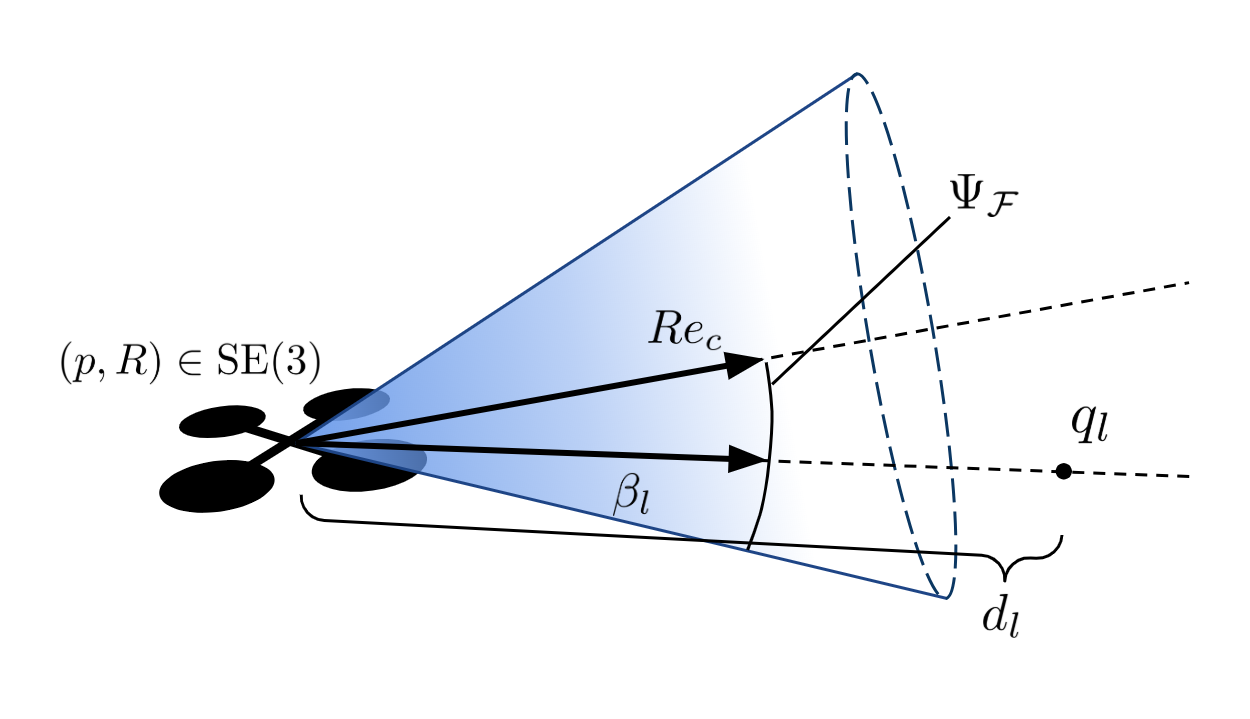
\includegraphics[width=0.8\linewidth]{fig/geometry.png}
\caption{特徴点観測の幾何学的条件}
\label{fig:geometry}
\end{figure}

\subsection{問題設定}

本研究の目的は,複数のエージェントが常に共通の特徴点を観測できるよう,各エージェントの制御入力を設計することである.具体的には,以下の問題を考える:

\begin{dfn}[共有視野保証問題]
エージェント集合$\mathcal{A}$と特徴点集合$\mathcal{L}$が与えられたとき,各エージェント$i \in \mathcal{A}$に対して,以下の条件を満たす制御入力$\xi_{B,i} = (\omega_i, v_{B,i})$を設計せよ:
\begin{enumerate}
\item 各エージェント$i$は目標位置$p_i^d$に向かって移動する.
\item 各エージェント$i$と$j$の間で,少なくとも$m$個の共通特徴点が常に観測可能である.つまり,$|\mathcal{C}_i \cap \mathcal{C}_j| \geq m$が常に成り立つ.
\end{enumerate}
\end{dfn}

この問題に対して,本研究では制御バリア関数(CBF)を用いたアプローチを提案する.特に,特徴点の可視性を確率的に評価し,CBFに組み込むことで,不確実性下でも安全な視野共有を実現する.また,非ホロノミックなドローンダイナミクスに対応するため,高次制御バリア関数(HOCBF)を導入し,分散最適化アルゴリズムにより各エージェントが局所的に制御入力を計算する枠組みを提案する.
